\iffalse
\let\negmedspace\undefined
\let\negthickspace\undefined
\documentclass[journal,12pt,twocolumn]{IEEEtran}
\usepackage{cite}
\usepackage{amsmath,amssymb,amsfonts,amsthm}
\usepackage{algorithmic}
\usepackage{graphicx}
\usepackage{textcomp}
\usepackage{xcolor}
\usepackage{txfonts}
\usepackage{listings}
\usepackage{enumitem}
\usepackage{mathtools}
\usepackage{gensymb}
\usepackage{comment}
\usepackage[breaklinks=true]{hyperref}
\usepackage{tkz-euclide} 
\usepackage{listings}
\usepackage{gvv}                                        
\def\inputGnumericTable{}                                 
\usepackage[latin1]{inputenc}                                
\usepackage{color}                                            
\usepackage{array}                                            
\usepackage{longtable}                                       
\usepackage{calc}                                             
\usepackage{multirow}                                         
\usepackage{hhline}                                           
\usepackage{ifthen}                                           
\usepackage{lscape}
\newtheorem{theorem}{Theorem}[section]
\newtheorem{problem}{Problem}
\newtheorem{proposition}{Proposition}[section]
\newtheorem{lemma}{Lemma}[section]
\newtheorem{corollary}[theorem]{Corollary}
\newtheorem{example}{Example}[section]
\newtheorem{definition}[problem]{Definition}
\newcommand{\BEQA}{\begin{eqnarray}}
\newcommand{\EEQA}{\end{eqnarray}}
\newcommand{\define}{\stackrel{\triangle}{=}}
\theoremstyle{remark}
\newtheorem{rem}{Remark}
\begin{document}
\parindent 0px
\bibliographystyle{IEEEtran}

\title{Assignment\\[1ex]10.5.4-2}
\author{ee23btech11215 - Penmetsa Srikar Varma$^{}$% <-this % stops a space
}
\maketitle
\newpage
\bigskip

\renewcommand{\thefigure}{\theenumi}
\renewcommand{\thetable}{\theenumi}
\section*{Question:}
Q10) The sum of three numbers in G.P. is 56. If we subtract 1, 7, 21 from these numbers in that order, we obtain an arithmetic progression. Find the numbers.
\section*{Solution:}
\fi
{\centering
Table of Parameters\\
}
\begin{table}[h]
    \centering
    \begin{tabular}{|c|c|}
        \hline
         Input Variable & Condition\\
        \hline
         $x\brak{0}$, $x\brak{n}$ & first term and general term of a GP\\
         \hline
         $r$ & common ratio of a GP\\
         \hline
         $x\brak{0},x\brak{1},x\brak{2}$ &three terms in GP \\
         \hline
           $x_i\brak{n}$ & general term of $\text{i}^{\text{th}}$ GP sequence\\
         \hline
           $x_i\brak{0}$ & first term of $\text{i}^{\text{th}}$ GP sequence\\
         \hline
           $r_i$ & common ratio of $\text{i}^{\text{th}}$ GP sequence\\
         \hline
    \end{tabular}

     \label{tab:t1}
\end{table}

$\brak{\text{n+1}}^{\text{th}}$ term of GP x\brak{n} is given by:
\begin{align}
\label{e1}
x\brak{n}&=x\brak{0}r^n\ u\brak{n}
\end{align}

Then from given table of parameters,
\begin{align}
x\brak{0}+x\brak{1}+x\brak{2}&=56
\end{align}

\begin{align}
\label{q2}
x\brak{0}\implies\frac{56}{\left(1+r+r^2\right)}
\end{align}

and from given another case following are in AP,
$$
x\brak{0}-1,x\brak{1}-7,x\brak{2}-21
$$

\begin{align}2(x\brak{1}-7)&=x\brak{0}-1+x\brak{2}-21\end{align}
\begin{align}x\brak{0}\left(r^2-2r+1\right)&=8\end{align}
and from (\ref{q2})
\begin{align}\frac{56.\left(r^2-2r+1\right)}{\left(1+r+r^2\right)}&=8\end{align}

\begin{align}
\label{q3}
r_1&=2\ ,\ r_2=\frac{1}{2}
\end{align}
so from (\ref{q2}),
\begin{align}x_1\brak{0}&=8\ ,\ x_2\brak{0}=32\end{align}
Then from (\ref{e1})
\begin{align}
    \label{a11}
    x_{1}\brak{n}&=8.2^{n}=2^{n+3}\ u\brak{n}
\end{align}
\begin{align}
    \label{a12}
    x_{2}\brak{n}=32.\left(\frac{1}{2}\right)^{n}u\brak{n}&=2^{5-n}\ u\brak{n}
\end{align}\\\\
$x_1\brak{0}$, $x_1\brak{1}$ and $x_1\brak{2}$ are 8, 16, 32 $\brak{or}$ $x_2\brak{0}$, $x_2\brak{1}$ and $x_2\brak{2}$ are 32, 16, 8 respectively
\begin{figure}[h]
    \centering
    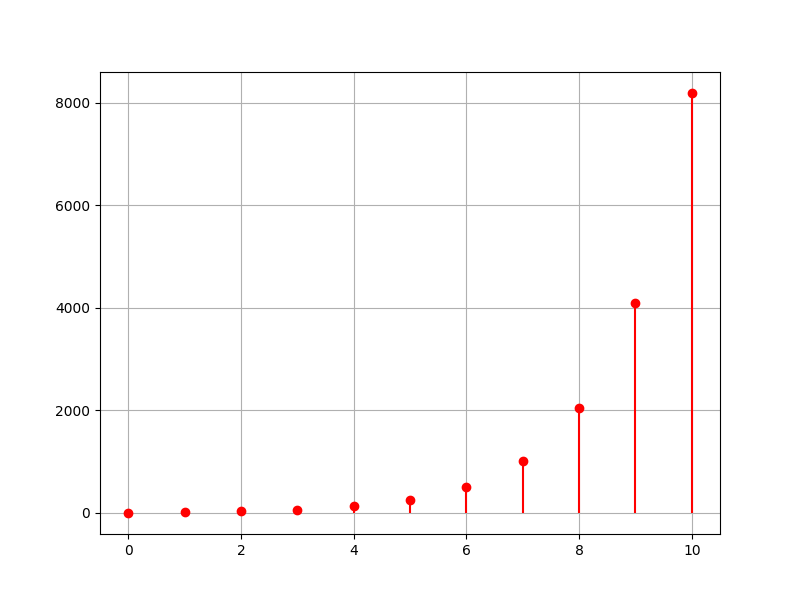
\includegraphics[scale=0.45]{ncert-maths/11/9/5/10/figs/py_1.png}
    \label{$2^{n+3}$}
\end{figure}

\begin{center}
    Graph of $x_1\brak{n}$
\end{center}
$z$-transform of $x_1\brak{n}$ is given by:\\
\begin{align}
\label{a13}
    X_1\brak{z}&=\sum_{k=-\infty}^{\infty} x_1\brak{k}.z^{-k}
\end{align}

from \brak{\ref{a11}},\\
\begin{align}X_1\brak{z}&=\sum_{k=0}^{\infty}2^{k+3}\ z^{-k}\end{align}

Hence,\\
\begin{align}
X_1\brak{z}&=\frac{8}{1-2z^{-1}},\quad |2z^{-1}|<1
\end{align}\\[10ex]

\begin{figure}[h]
    \centering
    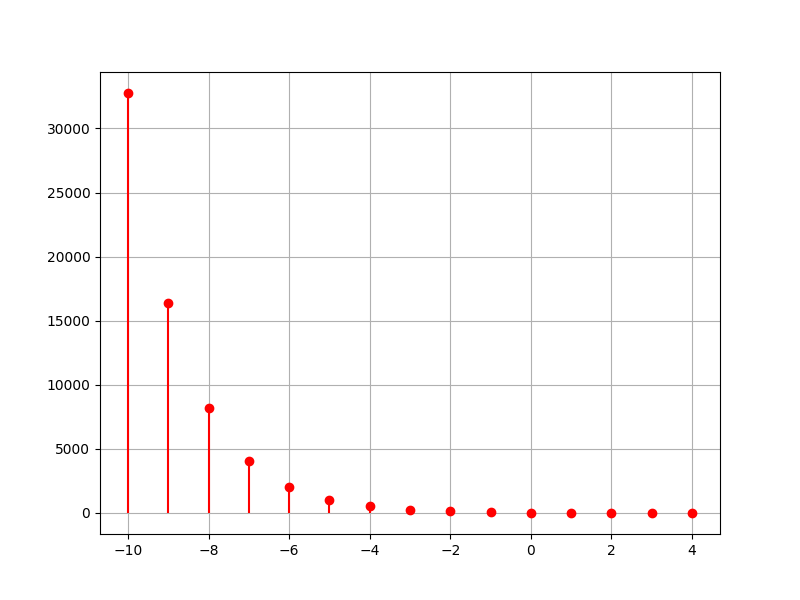
\includegraphics[scale=0.45]{ncert-maths/11/9/5/10/figs/py_2.png}
    \label{$2^{5-n}$}
\end{figure}

\begin{center}
    Graph of $x_2\brak{n}$
\end{center}

and also from \brak{\ref{a12}},\\
\begin{align}
    X_2\brak{z}&=\sum_{k=-\infty}^{\infty} x_2\brak{k}.z^{-k}
\end{align}
\begin{align}X_2\brak{z}&=\sum_{k=0}^{\infty} 2^{5-k}\ z^{-k}\end{align}

Hence,
\begin{align}X_2\brak{z}&=\frac{32}{1-{\brak{2z}^{-1}}},\quad |{\brak{2z}^{-1}}|<1 \end{align}

